\documentclass[10pt,a4paper]{article}
\usepackage[utf8]{inputenc}
\usepackage{array}
\usepackage{booktabs}
\usepackage{graphicx} 
\usepackage{amsmath}
\usepackage{amsfonts}
\usepackage{amssymb}
\usepackage{graphicx}



\title{
\includegraphics[width=2cm]{udacity-logo.png}\\We Rate Dogs: Act Report}
\date{March 2022}
\author{Tim Quan\\ \\ 
	\textit{\textbf{Udacity}: Data Analyst Nanodegree Program}\\ 
	\textit{\textbf{Project 03}: Wrangle and Analyze Data}}



\begin{document}
\maketitle

\section{Introduction}

    In this stage of the project, we used our previously gathered/wrangled data to interpret, analyze, come up with insights,
    and create visualizations.

    \section{Insights}
        \begin{itemize}
            \item Both favorite count and retweet count have a positive correlation with rating. We were able to establish this using OLS linear regression. 
            The associated p-values for both parameters were 0. It is likely that there is a pairwise relationship/multicollinarity between the two. We
            were able to visualize the pairwise relationship using the seaborn module.
            \begin{figure}[h]
                \centering
                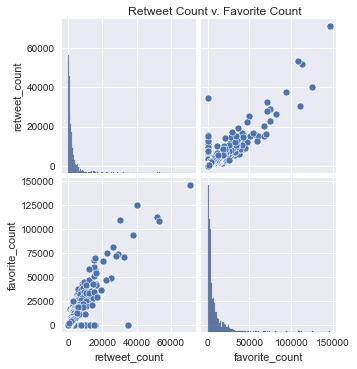
\includegraphics[width=0.5\textwidth]{../pairwise.jpg}            
                \caption{Retweet Count v. Favorite Count}
              \end{figure}
            \item Of the dog category/type, doggo and puppo records sufficient p-values to indicate that they have an impact rating; floofers and puppers do not.
            We were able to establish this using linear regression.
            \item The top 5 rated dogs (as detected) were pomeranian, Samoyed, golden retriever, kuvasz, great pyrenees, in that order. This rank order was limited to 
            breeds that had a minimum of 10 ratings to avoid being skewed by outliers/one off ratings.
        \end{itemize}
    \section{Visualizations}
        \begin{itemize}
            \item
                \begin{figure}[h]
                    \centering
                    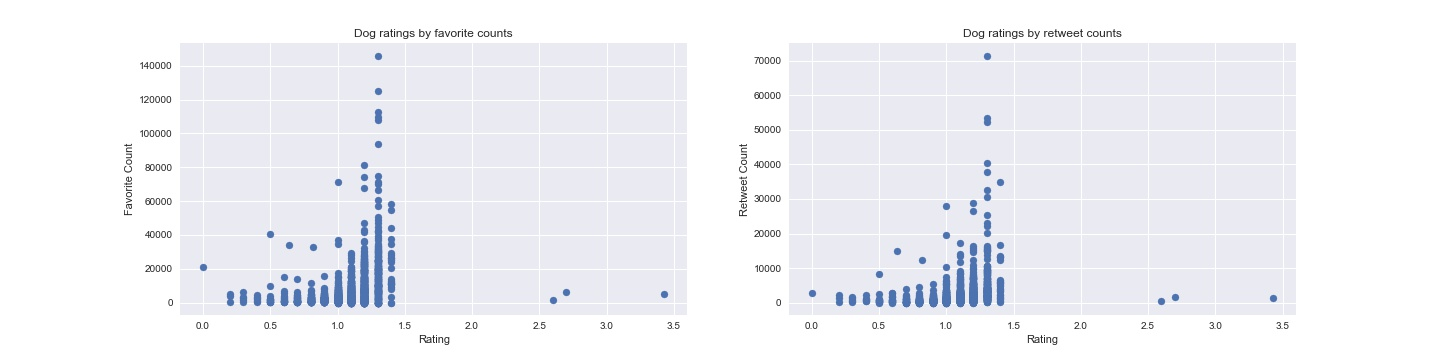
\includegraphics[width=1\textwidth]{scatter-retweets-favorites.jpg}            
                    \caption{Retweet Count v. Favorite Count}
                \end{figure}

        \end{itemize}



\end{document}